\documentclass[11pt]{article}
\usepackage[utf8]{inputenc}
\usepackage[english,italian]{babel} 
\usepackage{tikz}
\usepackage{tikz-3dplot} 
% Matematica
\usepackage{amsmath,amssymb,amsfonts,mathtools,mathrsfs}
% Grafica e immagini
\usepackage{graphicx} 
\usepackage{caption}
\usepackage{xcolor}
\usepackage{pgfplots}
\pgfplotsset{compat=1.18} 
\usepackage{tcolorbox}
\usepackage{listings}
\usepackage{hyperref}

% SINTASSI MACRO SFERA: #1=theta, #2=phi, #3=scala, #4=etichetta piano, #5=titolo vista, #6=label figura
\newcommand{\sfera}[6]{%
    \tdplotsetmaincoords{#1}{#2}% 
    \begin{tikzpicture}[tdplot_main_coords, scale=#3, >=stealth]
        
        % ==========================================================
        % CONFIGURAZIONE GENERALIZZATA
        % ==========================================================
        \def\R{1.2} % Raggio della sfera
        
        % Calcolo automatico del fattore di scala t = 2 / (1 - c)
        \pgfmathsetmacro{\tFACTOR}{2.0 / (1.0 - \coordC)}

        % Definizione geometrica dei punti nello spazio 3D automatizzata
        \coordinate (O) at (0,0,0);
        \coordinate (N) at (0,0,\R);
        \coordinate (P) at ({\coordA*\R}, {\coordB*\R}, {\coordC*\R}); 
        \coordinate (Pprime) at ({\tFACTOR*\coordA*\R}, {\tFACTOR*\coordB*\R}, -\R);

        % Piano z = -R proiettato in 3D
        \fill[gray!10, opacity=0.7] (-2,-2,-\R) -- (2,-2,-\R) -- (2,2,-\R) -- (-2,2,-\R) -- cycle;
        \draw[gray!50, dashed] (-2,-2,-\R) grid[step=0.5] (2,2,-\R);
        \draw[black!60, thick] (-2,-2,-\R) -- (2,-2,-\R) -- (2,2,-\R) -- (-2,2,-\R) -- cycle;
        \node[anchor=south west, font=\small] at (1.6,-1.8,-\R) {#4};

        % Asse z inferiore
        \draw[->,dashed] (0,0,-\R) -- (0,0,-1.8) node[anchor=north]{$z$};

        % SFERA 3D (Fissata sullo schermo)
        \begin{scope}[tdplot_screen_coords]
            \shadedraw[ball color=blue!15, opacity=0.25, draw=blue!50, thick] (0,0) circle (\R);
        \end{scope}

        % Equatore 3D
        \draw[blue!40, dashed, thick] (\R,0,0) arc (0:180:\R);
        \draw[blue!70, thick] (\R,0,0) arc (0:-180:\R);

        % Rette di proiezione
        \draw[red, thick] (N) -- (P);
        \draw[red, thick, dashed] (P) -- (Pprime);

        % Nodi
        \filldraw[black] (N) circle (0.6pt) node[anchor=south, font=\small] {$N$};
        \filldraw[black] (P) circle (0.6pt) node[anchor=south west, font=\small] {$P$};
        \filldraw[red] (Pprime) circle (0.8pt) node[anchor=north west, font=\small] {$P'$};
        \filldraw[gray] (O) circle (0.5pt) node[anchor=east, font=\small] {$O$};
    \end{tikzpicture}%
    \captionof{figure}{#5}\label{#6}
}

\begin{document}

% Configurazione dello stile per la visualizzazione del codice 
\lstset{
    language=[LaTeX]TeX,
    basicstyle={\ttfamily\small},
    keywordstyle={\color{blue!80!black}\bfseries},
    commentstyle={\color{green!50!black}\itshape},
    stringstyle={\color{orange}},
    backgroundcolor={\color{gray!5}},
    frame=single,
    rulecolor={\color{gray!30}},
    breaklines=true,
    showstringspaces=false,
    extendedchars=true,
    literate={~}{{\raisebox{0.5ex}{\texttildelow}}}{1}
}

\title{\textbf{La Proiezione Stereografica:\\Cenni Storici, Geometria e Aspetti Didattici}}
\author{}
\date{}
\maketitle

\section{Inquadramento Storico}

Oggi la proiezione stereografica è un argomento di grande interesse in diversi campi della matematica, dalla topologia alla geometry differenziale, fino all'analisi complessa. Ma se bisogna considerare le sue origini, queste risalgono a un contesto storico molto più antico e pratico, legato all'astronomia e alla cartografia. 

Nell'antica Grecia, la necessità di rappresentare la volta celeste su strumenti piani portò alla nascita di questa branca pratica della geometria, che permetteva agli astronomi di mappare le stelle e i pianeti senza dover affrontare la complessità della trigonometria sferica. Ipparco di Nicea (150-110 a.C.), uno dei più grandi astronomi dell'antichità viene accreditato come il primo a utilizzare la proiezione stereografica per calcolare le posizioni degli astri. Successivamente, Claudio Tolomeo (II secolo d.C.) formalizzò l'uso matematico di questa proiezione nel suo trattato \textit{Planisphaerium}, descrivendo il metodo per mappare la sfera celeste sul piano equatoriale.

\begin{figure}[htbp]
    \centering
    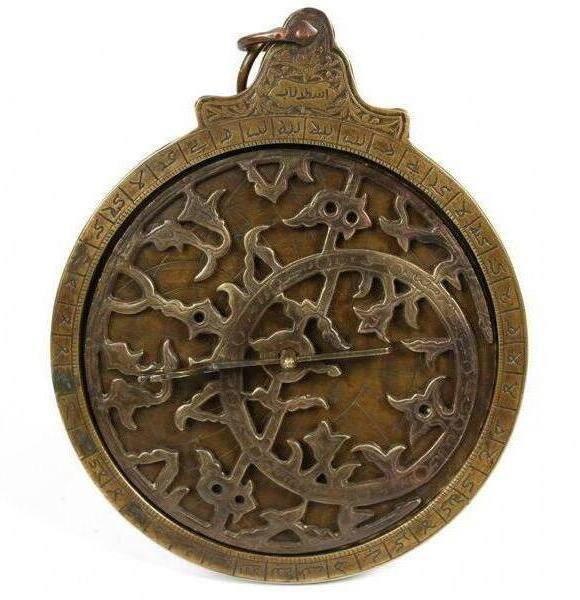
\includegraphics[width=0.5\textwidth]{astrolabio} 
    \caption{Foto di un \href{https://www.antik.it/Strumenti-astronomici-antichi/0000-Astrolabio-primi-1900/}{astrolabio} dei primi del 1900.}
    \label{fig:astrolabio}
\end{figure}

Questa intuizione geometrica costituì la base scientifica per lo sviluppo dell'astrolabio (Figura \ref{fig:astrolabio}), uno strumento di navigazione che ha dominato l'astronomia occidentale e islamica per oltre un millennio. Questo strumento consentiva di determinare l'ora, la latitudine e la posizione degli astri, sfruttando le proprietà della proiezione stereografica per rappresentare il cielo su un disco piatto. Il termine \textit{stereografica} (dal greco \textit{stereos}, solido, e \textit{graphia}, descrizione) venne coniato solo nel 1613 dal matematico gesuita François d'Aguilon (1561-1617) nel suo trattato \textit{Opticorum libri sex}. Nel XIX secolo, grazie ai lavori di Bernhard Riemann (1826-1866) e Ludwig Schli\"{a}fli (1814-1895), la proiezione diventò un pilastro della moderna geometria proiettiva e della teoria delle funzioni di variabile complessa (vedi \textit{Sfera di Riemann}).

\section{Aspetti Geometrici e Formalizzazione}
La proiezione stereografica è una mappa conforme che mette in corrispondenza biunivoca i punti di una sfera (privata del polo, punto $N$ di singolarità) con i punti di un piano affine. Consideriamo una sfera di raggio $R$ centrata nell'origine e proiettiamo dal Polo Nord $N=(0,0,R)$ sul piano affine tangente al Polo Sud ($\pi: z=-R$).

Dato un punto sulla sfera $P(x,y,z)$, le coordinate del punto proiettato $P'$ sul piano si ricavano imponendo la collinearità tra i punti $N$, $P$ e $P'$. Il sistema parametrico della retta passante per $N$ e $P$ è dato da:

\begin{equation}
\begin{cases}
X = t \cdot x \\
Y = t \cdot y \\
Z = R + t(z - R)
\end{cases}
\end{equation}
Imponendo la condizione di intersezione con il piano di proiezione $Z = -R$, si ricava il fattore di scala numerico $t$:
\begin{equation}
-R = R + t(z - R) \implies t = \frac{2R}{R - z}
\end{equation}

\section{Proprietà Geometriche e Approfondimenti Didattici}

La proiezione stereografica permette di esplorare proprietà geometriche fondamentali che la rendono uno strumento didattico utile per comprendere concetti avanzati in geometria e analisi complessa, legati alla conformità, alla gestione delle circonferenze e alla compattificazione topologica.

\subsection{Mappatura Conforme e Preservazione degli Angoli}
Una delle proprietà più rilevanti della proiezione stereografica è la sua \textbf{conformità}: vengono preservati gli angoli tra le curve. Se due curve sulla superficie della sfera si intersecano formando un angolo $\alpha$, le loro proiezioni sul piano $\pi$ si intersecheranno formando esattamente lo stesso angolo $\alpha$. Questa proprietà viene sfruttata nella cartografia (dove le bussole devono mantenere la direzione fedele, come nella proiezione di Mercatore) e nello studio delle mappe olomorfe.

\subsection{La Gestione delle Circonferenze}
Un'altra proprietà cruciale riguarda la corrispondenza delle curve sul piano:
\begin{itemize}
    \item Ogni circonferenza sulla sfera che non passa per il centro di proiezione $N$ viene mappata in una circonferenza sul piano $\pi$.
    \item Ogni circonferenza sulla sfera che passa per il polo di proiezione $N$ viene trasformata in una \textbf{retta} sul piano $\pi$.
\end{itemize}
Dal punto di vista proiettivo, una retta sul piano non è altro che una circonferenza di raggio infinito passante per il punto all'infinito.

\subsection{Il Compattamento di Aleksandrov e la Sfera di Riemann}
In ambito topologico, la proiezione offre la visualizzazione geometrica della compattificazione a un punto del piano reale $\mathbb{R}^2$. Mentre tutti i punti della sfera trovano un corrispettivo sul piano, il Polo Nord $N$ non si proietta in alcun punto finito. Tuttavia, se sul piano ci si allontana indefinitamente in qualsiasi direzione, l'immagine sulla sfera converge proprio verso il Polo Nord. Nel contesto dell'analisi complessa, questo permette di definire il piano complesso esteso $\mathbb{C}^* = \mathbb{C} \cup \{\infty\}$, modellizzato visivamente dalla \textbf{Sfera di Riemann}:
$$\mathbb{S}^2 \cong \mathbb{C} \cup \{\infty\}$$

\clearpage

\subsection{Metodo 1: Rappresentazione con TikZ Puro (2D)}
In questo primo approccio, la prospettiva è simulata geometricamente schiacciando l'asse verticale dell'ellisse equatoriale.

\begin{center}
\begin{tikzpicture}[scale=2.5, >=stealth]
    \def\R{1.2}
    \fill[gray!10, opacity=0.6] (-1.8,-1.5) -- (2.2,-1.5) -- (1.4,-0.5) -- (-2.6,-0.5) -- cycle;
    \draw[black!60, thick] (-1.8,-1.5) -- (2.2,-1.5) -- (1.4,-0.5) -- (-2.6,-0.5) -- cycle;
    \node[anchor=south west, font=\small] at (1.5,-1.5) {Piano $\pi: z=-R$};

    \draw[->, dashed, black!60] (0,-1.2) -- (0,-1.8) node[anchor=north] {$z$};
    \draw[dashed, black!40] (0,0) -- (0,-1.2);

    \shadedraw[ball color=blue!15, opacity=0.25, draw=blue!60, thick] (0,0) circle (\R);

    \draw[blue!40, dashed, thick] (\R,0) arc (0:180:{\R} and 0.35); 
    \draw[blue!70, thick] (\R,0) arc (0:-180:{\R} and 0.35); 

    \coordinate (O) at (0,0);
    \coordinate (N) at (0,\R);                        
    \coordinate (P) at (0.6,0.3);                      
    \coordinate (Pprime) at (1.6,-1.2);              

    \draw[red, thick] (N) -- (P);
    \draw[red, thick, dashed] (P) -- (Pprime);
    \draw[gray!40, dashed] (0,0) -- (0.6,0.3); 

    \filldraw[black] (N) circle (0.6pt) node[anchor=south, font=\small] {$N$};
    \filldraw[black] (P) circle (0.6pt) node[anchor=south west, font=\small] {$P$};
    \filldraw[red] (Pprime) circle (0.8pt) node[anchor=north west, font=\small] {$P'$};
    \filldraw[gray] (O) circle (0.5pt) node[anchor=east, font=\small] {$O$};
\end{tikzpicture}
\end{center}

\clearpage

\subsection{Metodo 2: Rappresentazione con \texttt{tikz-3dplot} (3D)}
\begin{figure}[htbp] 
    \centering

    % 1. PRIMA FIGURA: VISTA ASSONOMETRICA (Scala ridotta a 1.6 per fare spazio)
    \def\coordA{0.7}
    \def\coordB{0.5}
    \def\coordC{0.51}
    \sfera{70}{110}{1.6}{Piano $\pi: z = -R$}{Vista Assonometrica Standard}{fig:assonometrica}
    
    \vspace{1.5em} % Un po' di spazio verticale controllato tra sopra e sotto

    % 2. SECONDA E TERZA FIGURA AFFIANCATE (Scala ridotta a 1.25 per non uscire dai margini)
    \def\coordA{0.6}
    \def\coordB{0.3}
    \def\coordC{-0.2}
    
    \begin{minipage}[t]{0.48\textwidth}
        \centering
        \sfera{90}{0}{1.25}{$\pi$}{Vista Laterale}{fig:laterale}
    \end{minipage}% <--- Questo commento neutralizza lo spazio vuoto e incolla la minipage successiva
    \hfill
    \begin{minipage}[t]{0.48\textwidth}
        \centering
        \sfera{0}{0}{1.25}{$\pi$}{Vista Zenitale}{fig:zenitale}
    \end{minipage}

\end{figure}

\clearpage

\section*{Appendice: Codici Sorgenti TikZ}

\subsection*{Sorgente Metodo 1: TikZ Puro (2D)}
\begin{lstlisting}
\begin{tikzpicture}[scale=2.5, >=stealth]
    
    % 1. PARAMETRI E GEOMETRIA FISSA

    \def\R{1.2} % Raggio della sfera
    
    % Definizione manuale dei punti allineati (Ottimizzati per la vista 2D)
    \coordinate (O)      at (0,0);
    \coordinate (N)      at (0,\R);
    \coordinate (P)      at (0.6,0.3);
    \coordinate (Pprime) at (1.6,-1.2); 
    
    % 2. AMBIENTE CIRCOSTANTE (Piano di proiezione pi e Assi)

    % Disegno del piano affine inclinato pi: z = -R
    \fill[gray!10, opacity=0.6] (-1.8,-1.5) -- (2.2,-1.5) -- (1.4,-0.5) -- (-2.6,-0.5) -- cycle;
    \draw[black!60, thick]     (-1.8,-1.5) -- (2.2,-1.5) -- (1.4,-0.5) -- (-2.6,-0.5) -- cycle;
    \node[anchor=south west, font=\small] at (1.5,-1.5) {Piano $\pi: z=-R$};
    
    % Prolungamento tratteggiato dell'asse verticale z
    \draw[dashed, black!40] (0,0) -- (0,-1.2);
    \draw[->, dashed, black!60] (0,-1.2) -- (0,-1.8) node[anchor=north] {$z$};
    
    
    % 3. RAPPRESENTAZIONE DELLA SFERA ED EQUATORE SHIACCIATO
    
    % Ombreggiatura della sfera bidimensionale
    \shadedraw[ball color=blue!15, opacity=0.25, draw=blue!60, thick] (0,0) circle (\R);
    
    % Equatore simulato tramite ellisse (Retro nascosto e Fronte visibile)
    \draw[blue!40, dashed, thick] (\R,0) arc (0:180:{\R} and 0.35); 
    \draw[blue!70, thick]        (\R,0) arc (0:-180:{\R} and 0.35); 
    
    % Raggio vettore di supporto interno alla sfera
    \draw[gray!40, dashed] (0,0) -- (0.6,0.3); 
    
    
    % 4. RETTE DI PROIEZIONE E NODI DI TESTO
    
    % Rette di proiezione stereografica (N-P-P')
    \draw[red, thick]        (N) -- (P);
    \draw[red, thick, dashed] (P) -- (Pprime);
    
    % Posizionamento dei nodi sui punti geometrici
    \filldraw[black] (N)      circle (0.6pt) node[anchor=south, font=\small]      {$N$};
    \filldraw[black] (P)      circle (0.6pt) node[anchor=south west, font=\small] {$P$};
    \filldraw[red]   (Pprime) circle (0.8pt) node[anchor=north west, font=\small] {$P'$};
    \filldraw[gray]  (O)      circle (0.5pt) node[anchor=east, font=\small]       {$O$};
    
\end{tikzpicture}
\end{lstlisting}

\subsection*{Sorgente Metodo 2: Macro Dinamica Estesa ed Automatizzata}
\begin{lstlisting}
\newcommand{\sfera}[6]{%
    \tdplotsetmaincoords{#1}{#2}%
    \begin{tikzpicture}[tdplot_main_coords, scale=#3, >=stealth]
        
        
        % 1. PARAMETRI E CALCOLI GEOMETRICI
        
        \def\R{1.2} % Raggio della sfera
        
        % Calcolo automatico del fattore di scala t = 2 / (1 - z)
        \pgfmathsetmacro{\tFACTOR}{2.0 / (1.0 - \coordC)}
        
        % Definizione delle coordinate 3D dei punti analitici
        \coordinate (O)      at (0,0,0);
        \coordinate (N)      at (0,0,\R);
        \coordinate (P)      at ({\coordA*\R}, {\coordB*\R}, {\coordC*\R}); 
        \coordinate (Pprime) at ({\tFACTOR*\coordA*\R}, {\tFACTOR*\coordB*\R}, -\R);
        
        
        % 2. AMBIENTE CIRCOSTANTE (Piano di proiezione e Assi)
        
        % Griglia e riempimento del piano pi: z = -R
        \fill[gray!10, opacity=0.7] (-2,-2,-\R) -- (2,-2,-\R) -- (2,2,-\R) -- (-2,2,-\R) -- cycle;
        \draw[gray!50, dashed]     (-2,-2,-\R) grid[step=0.5] (2,2,-\R);
        \draw[black!60, thick]     (-2,-2,-\R) -- (2,-2,-\R) -- (2,2,-\R) -- (-2,2,-\R) -- cycle;
        
        % Etichetta del piano e prolungamento asse z
        \node[anchor=south west, font=\small] at (1.6,-1.8,-\R) {#4};
        \draw[->, dashed] (0,0,-\R) -- (0,0,-1.8) node[anchor=north]{$z$};
        
        
        % 3. RAPPRESENTAZIONE DELLA SFERA ED EQUATORE
        
        % Ombreggiatura della sfera 3D (fissata in coordinate schermo)
        \begin{scope}[tdplot_screen_coords]
            \shadedraw[ball color=blue!15, opacity=0.25, draw=blue!50, thick] (0,0) circle (\R);
        \end{scope}
        
        % Tratteggio dell'equatore (retro nascosto e fronte visibile)
        \draw[blue!40, dashed, thick] (\R,0,0) arc (0:180:\R);
        \draw[blue!70, thick]        (\R,0,0) arc (0:-180:\R);
        
        
        % 4. VETTORI E RETTE DI PROIEZIONE STEREOGRAFICA
        
        \draw[red, thick]        (N) -- (P);       % Tratto continuo interno
        \draw[red, thick, dashed] (P) -- (Pprime); % Tratto esterno tratteggiato
        
    \end{tikzpicture}%
    \captionof{figure}{#5}\label{#6}
}
\end{lstlisting}

\clearpage

\begin{thebibliography}{999}
\bibitem{1} C. Tolomeo, \textit{Planisphaerium}, II secolo d.C.
\bibitem{2} F. d'Aguilon, \textit{Opticorum libri sex}, 1613.
\bibitem{3} B. Riemann, \textit{Grundlagen für eine allgemeine Theorie...}, 1851.
\bibitem{4} T. Needham, \textit{Visual Complex Analysis}, 1997.
\bibitem{5} H. S. M. Coxeter, \textit{Introduction to Geometry}, 2003.
\bibitem{6} \href{https://catalogo.museogalileo.it/approfondimento/Astrolabio.html}{\textit{Astrolabio}}, Museo Galileo, Firenze.
\end{thebibliography}
\end{document}